% !TEX root = ../main.tex
\section{Неперервні випадкові вектори}

\begin{definition}
    Вимірна функція $\xi(\omega): \Omega \rightarrow \mathbb{R}^n$ називається 
    \emph{неперервним випадковим вектором}, якщо координати $\xi_i$ є 
    неперервними випадковими величинами для $i = 1,...,n$.
\end{definition}
Функція розподілу $F_{\vec{\xi}}\left(\vec{x}\right) = 
P\left\{\omega:\xi_1(\omega)<x_1,...,\xi_n(\omega)<x_n\right\}$ є неперервною по всім аргументам.

\subsection{Щільність розподілу двовимірного неперервного випадкового вектора}
\begin{definition}
    \emph{Щільністю розподілу} двовимірного випадкового вектора називається 
    подвійна границя
    \begin{equation}
        f_{\vec{\xi}}(x, y) = \lim_{\substack{\Delta x \to 0 \\ 
        \Delta y \to 0}} \frac{P\left\{\vec{\xi} \in \Pi\right\}}
        {\Delta x \Delta y}
    \end{equation}
    де $\Pi = \left[x; x+\Delta x\right] \times \left[y; y+\Delta y\right]$.
\end{definition}
\begin{remark}
    В означенні 1 замість можна брати будь-яку обмежену замкнену область (компакт) 
    $D$ і тоді
    \begin{equation*}
        f_{\vec{\xi}}(x, y) = \lim_{S(D) \to 0} 
        \frac{P\left\{\vec{\xi} \in D\right\}}
        {S(D)}
    \end{equation*}
\end{remark}

\noindent\textbf{Зв’язок щільності розподілу з сумісною функцією розподілу: }
\begin{gather*}
    \lim_{\substack{\Delta x \to 0 \\ 
\Delta y \to 0}} \frac{P\left\{\vec{\xi} \in \Pi\right\}}
{\Delta x \Delta y} = 
\lim_{\substack{\Delta x \to 0 \\ \Delta y \to 0}} 
\left(
    \frac{F_{\vec{\xi}}(x+\Delta x, y+\Delta y) - F_{\vec{\xi}}(x, y+\Delta y)}
    {\Delta x \Delta y}
    -
    \frac{F_{\vec{\xi}}(x+\Delta x, y) - F_{\vec{\xi}}(x, y)}
    {\Delta x \Delta y}
\right) = \\
= \left[\text{формула Лагранжа про скінченні прирости}, \theta_1, \theta_2 \in (0, 1)\right] = \\
= \lim_{\substack{\Delta x \to 0 \\ \Delta y \to 0}} 
\left(
    \frac{\frac{\partial F}{\partial x}(x + \theta_1 \Delta x, y + \Delta y)\Delta x}
    {\Delta x \Delta y}
    -
    \frac{\frac{\partial F}{\partial x}(x + \theta_2 \Delta x, y)\Delta x}
    {\Delta x \Delta y}
\right) =  \\
= \left[\theta_3, \theta_4 \in (0, 1)\right] 
= \lim_{\substack{\Delta x \to 0 \\ \Delta y \to 0}}
\frac{\frac{\partial^2 F}{\partial x \partial y}(x + \theta_3 \Delta x, 
y + \theta_4 \Delta y)\Delta y}
{\Delta y} = \frac{\partial^2 F_{\vec{\xi}}}{\partial x \partial y}(x, y)\end{gather*}

Таким чином, якщо існує неперервна $ \frac{\partial^2 F_{\vec{\xi}}}{\partial x \partial y}$, то
\begin{equation}\label{eq:dens_r2}
    f_{\vec{\xi}}(x, y) = \frac{\partial^2 F_{\vec{\xi}}}{\partial x \partial y}(x, y)
\end{equation}

\begin{definition}
    Поверхня, що є графіком щільності двовимірного випадкового вектора називається 
    \emph{поверхнею розподілу}.
\end{definition}
\begin{definition}
    Лінії, де $f_\xi(x, y) = const$, називаються \emph{лініями рівних ймовірностей}.
\end{definition}

\noindent\textbf{Властивості щільності: }

\begin{enumerate}
    \item $f_{\vec{\xi}}(x, y) \geq 0$.
    \item З формули \refeq{eq:dens_r2}: $F_{\vec{\xi}}(x, y) 
    = \int\limits_{-\infty}^x \int\limits_{-\infty}^y f_{\vec{\xi}}(t, s) 
    dt ds $.
    \item Умова нормування: 
    $\int\limits_{-\infty}^{+\infty} \int\limits_{-\infty}^{\infty} f_{\vec{\xi}}(t, s) 
    dt ds = 1$ --- об'єм під поверхнею розподілу 
    дорівнює 1.
    \item $F_{\xi_1}(x) = \int\limits_{-\infty}^{x} \int\limits_{-\infty}^{+\infty} 
    f_{\vec{\xi}}(t, s) dt ds$.

    $F_{\xi_2}(y) = \int\limits_{-\infty}^{+\infty} \int\limits_{-\infty}^{y} 
    f_{\vec{\xi}}(t, s) dt ds$.
    \item Щільності розподілу окремих координат називаються 
    \emph{маргінальними щільностями}.

    $f_{\xi_1}(x) = F'_{\xi_1}(x) 
    = \int\limits_{-\infty}^{+\infty} f_{\vec{\xi}}(x, y) dy $.

    $f_{\xi_2}(y) = F'_{\xi_2}(y) 
    = \int\limits_{-\infty}^{+\infty} f_{\vec{\xi}}(x, y) dx $.
    
    \item D --- замкнена обмежена область в $\mathbb{R}^2$.
    $P\left\{ \vec{\xi} \in D \right\} = \iint\limits_D f_{\vec{\xi}}(x, y) 
    dx dy$.
\end{enumerate}

\subsection{Рівномірний закон розподілу на площині}
\begin{definition}
    D --- замкнена обмежена область в $\mathbb{R}^2$. 
    Вектор $\vec{\xi} = (\xi_1,\xi_2)^T$ називається 
    \emph{рівномірно розподіленим в області D}, якщо 
    \begin{equation*}
        f_{\vec{\xi}}(x, y) = 
        \begin{cases}
            \frac{1}{S(D)},&(x, y) \in D \\
            0,&(x, y) \notin D
        \end{cases}
    \end{equation*}
\end{definition}
\begin{example}
    \begin{tabular}{c m{4cm}}
        $f_{\vec{\xi}}(x, y) = 
        \begin{cases}
            2, & (x, y) \in D \\
            0, & (x, y) \notin D
        \end{cases}
        $
        &
        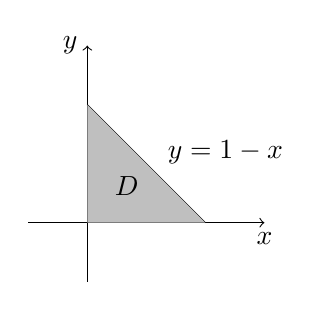
\begin{tikzpicture}[scale = 1.5]
            \draw [->] (0, -0.5) -- (0, 1.5);
            \draw [->] (-0.5, 0) -- (1.5, 0);
            \draw (1, 0) -- (0, 1);
            \fill [lightgray] (0, 0) -- (1, 0) -- (0, 1);
            \node [below] at (1.5, 0) {$x$};
            \node [left] at (0, 1.5) {$y$};
            \node [above right] at (0.15, 0.15) {$D$};
            \node [right] at (0.6, 0.6) {$y = 1 - x$};
        \end{tikzpicture}
    \end{tabular}
    
    \begin{enumerate}
        \item $f_{\xi_1}(x) = \int\limits_{-\infty}^{+\infty} f_{\vec{\xi}}(x, y) dy = 
        \begin{cases}
            0 , &x\leq0 \text{ або } x>1\\
            \int\limits_0^{1-x} 2 dy = 2(1-x), & 0 < x \leq 1 
        \end{cases}$

        $f_{\xi_2}(y) = \int\limits_{-\infty}^{+\infty} f_{\vec{\xi}}(x, y) dx = 
        \begin{cases}
            0 , &y\leq0 \text{ або } y>1\\
            \int\limits_0^{1-y} 2 dx = 2(1-y), & 0 < y \leq 1 
        \end{cases}$
        \item Функції розподілу координат: 
        
        $F_{\xi_1}(x) = \int\limits_{-\infty}^{x} f_{\xi_1}(t) dt = \begin{cases}
            0, & x\leq 0 \\
            2\int\limits_0^x (1-t) dt = 2(x-\frac{x^2}{2}) = 2x - x^2, & 0<x\leq 1 \\
            1, x>1
        \end{cases}$
        
        $F_{\xi_2}(y) = \int\limits_{-\infty}^{y} f_{\xi_2}(t) dt = \begin{cases}
            0, & y\leq 0 \\
            2y - y^2, & 0<y\leq 1 \\
            1, y>1
        \end{cases}$
        \item Сумісна функція розподілу: 
        
        $F_{\vec{\xi}}(x, y) = 
        \int\limits_{-\infty}^{x} \int\limits_{-\infty}^{y} 
        f_{\vec{\xi}}(t, \tau) dt d\tau$

        \begin{enumerate}[label=(\Roman*)]
            \item $(x, y) \in D_0$
            
            $D_0 = \left\{(x, y):\; x \leq 0 \lor y \leq 0\right\}$

            $F_{\vec{\xi}}(x, y) = 0$

            \item $(x, y) \in D_1$
            
            $D_1 = \left\{(x, y):\; x \in \left[0, 1\right],
            y \in \left[0, 1-x\right]\right\}$

            $F_{\vec{\xi}}(x, y) = 2xy$

            \item $(x, y) \in D_2$
            
            $D_2 = \left\{(x, y):\; x \in \left[0, 1\right],
            y \in \left[1-x, 1\right]\right\}$

            $F_{\vec{\xi}}(x, y) = 2(xy - \frac{1}{2}(x-1+y)(y-1+x))$

            \item $(x, y) \in D_3$
            
            $D_3 = \left\{(x, y):\; x > 1,
            y \in \left[0, 1\right]\right\}$

            $F_{\vec{\xi}}(x, y) = 2\frac{1+1-y}{2}y = y(2-y)$

            \item $(x, y) \in D_4$
            
            $D_4 = \left\{(x, y):\; y > 1,
            x \in \left[0, 1\right]\right\}$

            $F_{\vec{\xi}}(x, y) = 2\frac{1+1-x}{2}x = x(2-x)$

            \item $(x, y) \in D_5$
            
            $D_5 = \left\{(x, y):\; x > 1 \land y > 1\right\}$

            $F_{\vec{\xi}}(x, y) = 1$
        \end{enumerate}
        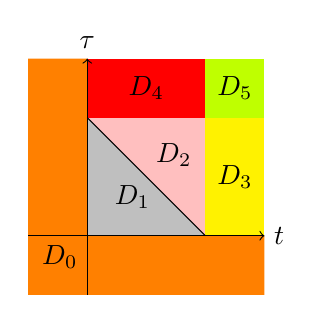
\begin{tikzpicture}[scale = 1.5]
            \fill [orange] (-0.5, -0.5) -- (-0.5, 1.5) -- (0, 1.5) --
                           (0, 0) -- (1.5, 0) -- (1.5, -0.5) -- (-0.5, -0.5);
            \fill [lightgray] (0, 0) -- (1, 0) -- (0, 1);
            \fill [pink] (0, 1) -- (1, 0) -- (1, 1);
            \fill [red] (0, 1) rectangle (1, 1.5);
            \fill [yellow] (1, 0) rectangle (1.5, 1);
            \fill [lime] (1, 1) rectangle (1.5, 1.5);
            \draw [->] (0, -0.5) -- (0, 1.5);
            \draw [->] (-0.5, 0) -- (1.5, 0);
            \draw (1, 0) -- (0, 1);
            \node [right] at (1.5, 0) {$t$};
            \node [above] at (0, 1.5) {$\tau$};
            \node [below left] at (0, 0) {$D_0$};
            \node [above right] at (0.15, 0.15) {$D_1$};
            \node [above right] at (0.5, 0.5) {$D_2$};
            \node at (0.5, 1.25) {$D_4$};
            \node at (1.25, 0.5) {$D_3$};
            \node at (1.25, 1.25) {$D_5$};
        \end{tikzpicture}
    \end{enumerate}
\end{example}

\begin{remark}
    Перевірити правильність побудови функції розподілу можна за допомогою 
    умови узгодженості, перевірки точок стику та неперервності на лініях стику.
\end{remark}

\subsection{Щільність розподілу n-вимірного неперервного випадкового 
вектора}
\begin{definition}
    $\vec{\xi} = \left(\xi_1, \xi_2, ..., \xi_n\right)^T,\; \Pi = 
    \left[x_1; x_1+\Delta x_1\right] \times ... \times 
    \left[x_n; x_n+\Delta x_n\right]$
    \emph{Щільністю розподілу} n-вимірного неперервного випадкового 
    вектора називається границя
    \begin{equation*}
        f_{\vec{\xi}} (\vec{x}) = \lim_{\substack{\Delta x_i \to 0 \\
        \forall i = \overline{1,n}}} 
        \frac{P\left\{\vec{\xi} \in \Pi\right\}}{\Delta x_1...\Delta x_n}
    \end{equation*}

    Якщо існує і неперервна $\frac{\partial^n F_{\vec{\xi}}(\vec{x})}
    {\partial x_1 ... \partial x_n}$, то
    \begin{equation*}
        f_{\vec{\xi}} (\vec{x}) = \frac{\partial^n F_{\vec{\xi}}}
        {\partial x_1 ... \partial x_n}(\vec{x})
    \end{equation*}
\end{definition}

\noindent \textbf{Властивості}
\begin{enumerate}
    \item $f_{\vec{\xi}}(\vec{x}) \geq 0$
    \item $\int\limits_{-\infty}^{+\infty}...\int\limits_{-\infty}^{+\infty}
    f_{\vec{\xi}} (\vec{x})dx_1...dx_n = 1$
    \item $F_{\vec{\xi}}(\vec{x}) = 
    \int\limits_{-\infty}^{x_1}...\int\limits_{-\infty}^{x_n}
    f_{\vec{\xi}} (\vec{t})dt_1...dt_n$
    \item $F_{\xi_1\xi_2...\xi_k}(x_1, ..., x_k) = 
    \int\limits_{-\infty}^{x_1}...\int\limits_{-\infty}^{x_k}
    \int\limits_{-\infty}^{+\infty}...\int\limits_{-\infty}^{+\infty}
    f_{\vec{\xi}} (\vec{t})dt_1...dt_n$

    $F_{\xi_i}(x_i) = \int\limits_{-\infty}^{+\infty}...
    \int\limits_{-\infty}^{x_i}...\int\limits_{-\infty}^{+\infty}
    f_{\vec{\xi}} (\vec{t})dt_1...dt_n$

    \item $f_{\xi_1...\xi_k}(x_1, ..., x_k) = 
    \underbrace{
        \int\limits_{-\infty}^{+\infty} 
        ... 
        \int\limits_{-\infty}^{+\infty}
    }_{n-k} f_{\vec{\xi}}(\vec{x}) dx_{k+1}..dx_n$
    \item D - замкнена обмежена область в $\mathbb{R}^n$ (компакт).
    
    $P\left\{\vec{\xi} \in D\right\} = {\int\int...\int}_D f_{\vec{\xi}}(\vec{x})
    dx_1 ... dx_n$
\end{enumerate}
\begin{exercise}
    Довести властивості.
\end{exercise}

\subsection{Незалежні випадкові величини}
\begin{definition}
    $\xi_1$ та $\xi_2$ називаються незалежними, якщо 
    $\forall x, y \in \mathbb{R}$:  
    $\left\{\omega\;:\;\xi_1 < x\right\}$ та $\left\{\omega\;:\;\xi_2 < y\right\}$ ---
    незалежні (як події).
\end{definition}
\begin{remark}
    Якщо $\xi_1$, $\xi_2$ - незалежні координати випадкового вектора $\vec{\xi}$, 
    то $F_{\vec{\xi}}(x, y) = 
    P\left(\left\{\xi_1 < x\right\} \cap \left\{\xi_2 < y\right\}\right) = 
    F_{\xi_1}(x)F_{\xi_2}(y)$.

    Якщо ж вектор ще й є неперервним випадковим вектором та існує неперервна 
    друга часткова похідна, то
    $f_{\vec{\xi}}(x, y) = \frac{\partial^2 F_{\vec{\xi}}(x, y)}
    {\partial x \partial y} = \frac{\partial^2(F_{\xi_1}(x)F_{\xi_2}(y))}{\partial x \partial y} 
    = F_{\xi_1}^\prime (x)F_{\xi_2}^\prime (y) = 
    f_{\xi_1}(x)f_{\xi_2}(y)$.
\end{remark}